%!TEX root = <main.tex>
\section{Preliminaries and Overview}\label{sec:preliminaries}
In this section first we formally state the problem and explain our assumptions.
Then we formalize the internals of some of the layers in a Deep CNN for the purpose of proposing our incremental inference approach in Section 4. Finally we briefly explain the Structural Similarity Index (SSIM) which is used to quantify the quality of the generated sensitivity heat map with respect to the original in the context of approximate inference.

\subsection{Problem Statement and Assumptions}

\begin{table}[t]
  \centering
  \caption{Symbols used in the Preliminaries Section}
  \scalebox{0.8}{\begin{tabular}{p{2cm}p{7.5cm}}
    \toprule
    \textbf{Symbol} & \textbf{Meaning}\\
    \midrule \midrule
    $\mathcal{I} (\mathcal{I}_{img})$ & Input activation volume (Input Image)\\
    \midrule
    $\mathcal{O}$ & Output activation volume\\
    \midrule
    $C_{\mathcal{I}},H_{\mathcal{I}},W_{\mathcal{I}}$ & Depth, height, and width of Input\\
    \midrule
    $C_{\mathcal{O}},H_{\mathcal{O}},W_{\mathcal{O}}$ & Depth, height, and width of Output\\
    \midrule
    $\mathcal{K}_{conv}$ & Convolution filter kernels\\
    \midrule
    $\mathcal{B}_{conv}$ & Convolution bias value vector\\
    \midrule
    $\mathcal{K}_{pool}$ & Pooling filter kernel\\
    \midrule
    $H_{\mathcal{K}},W_{\mathcal{K}}$ & Height and width of filter kernel\\
    \midrule
    $S (S_x,S_y)$ & Filter kernel or occlusion patch striding amount ($S_x$ and $S_y$ corresponds to width and height dimensions)\\
    \midrule
    $P (P_x,P_y)$ & Padding amount ($P_x$ and $P_y$ corresponds to padding along width and height dimensions)\\
    \midrule
    $Q (Q_{inc})$ & Total FLOPS count with full (incremental) inference\\
    \midrule
    $L$ & Set of convolution layers in a CNN\\
    \midrule
    $\mathcal{P}$ & Occluding patch\\
    \midrule
    $\mathcal{I}^{x,y}_{img}$ & Modified image by superimposing $\mathcal{P}$ on top of $\mathcal{I}_{img}$ such that the top left corner of $\mathcal{P}$ is positioned at $x,y$ location of $\mathcal{I}_{img}$\\
    \midrule
    $M$ & Heat map produced by the occlusion experiment\\
    \midrule
    $H_M,W_M$ & Height and width of $M$\\
    \midrule
    $f$ & Fine-tuned CNN\\
    \midrule
    $C$ & Class label predicted by $f$ for the original image $\mathcal{I}_{img}$\\
    \midrule
    $\bm\circ_{x,y}$ & Superimposition operator. $A~\circ_{x,y}~B$, superimposes $B$ on top of $A$ starting off at $(x,y)$ position\\
    \bottomrule
  \end{tabular}}
\label{table:preliminaries_symbols}
\end{table}


We are given a fine-tuned CNN $f$, an image $\mathcal{I}_{img}$ on which the occlusion experiment needs to be run, the predicted class label $C$ for the image $\mathcal{I}_{img}$, an occluding patch $\mathcal{P}$ in RGB format, and patch striding amounts $S_{x}$ and $S_{y}$ which will be used to move the occlusion patch on the image at a time in horizontal and vertical directions. The occlusion experiment workload is to generate a 2D heat map $M$ where each individual value in $M$ corresponds to the predicted probability for $C$ by $f$ when $\mathcal{P}$ is superimposed on $\mathcal{I}_{img}$ corresponding to the position of that particular value. More precisely, we can state the workload using the following set of logical statements:


\begin{align}
\label{eqn:mheight}
W_M =&~ \lfloor(\texttt{width}(\mathcal{I}_{img}) - \texttt{width}(\mathcal{P}) + 1)/S_{x}\rfloor\\
\label{eqn:mwidth}
H_M =&~ \lfloor(\texttt{height}(\mathcal{I}_{img}) - \texttt{height}(\mathcal{P}) + 1)/S_{y}\rfloor\\
M \in&~ \mathcal{\rm I\!R}^{H_M \times W_M}\\
\forall~ x,y \in&~ [0, H_M] \times [0, W_M]:\\
\label{eqn:patchimpose}
& \mathcal{I}_{img}^{x,y} \leftarrow ~\mathcal{P} ~ \bm\circ_{x,y} ~ \mathcal{I}_{img}\\
\label{eqn:outputval}
& M[x,y] \leftarrow f(\mathcal{I}_{img}^{x,y},C)
\end{align}

Step (\ref{eqn:mheight}), and (\ref{eqn:mwidth}) calculates the dimensions of the generated heat map $M$ which is dependent on the dimensions of $\mathcal{I}_{img}$, $P$, and the values of $S_{x}$ and $S_{y}$.
Step (\ref{eqn:patchimpose}) superimposes $\mathcal{P}$ on $\mathcal{I}_{img}$ with its top left corner placed on the (x,y) location of $\mathcal{I}_{img}$.
Step (\ref{eqn:outputval}) calculates the output value at the (x,y) location by performing CNN inference for $\mathcal{I}_{img}^{x,y}$ using $f$ and taking the predicted probability for the label $C$.

We make few simplifying assumptions in this paper for tractability sake.
First we assume that $f$ is a fine-tuned CNN from a roaster of well-known CNNs (currently, VGG, ResNet, and Inception).
This is a reasonable start, since most recent fine-tuning based transfer learning applications used only such well-known CNNs from model zoos \cite{caffemodelzoo, tfmodelzoo}.
Nevertheless, our work is orthogonal to the specifics of a particular architecture and the proposed approaches can be easily extended to any architecture.
We leave support for arbitrary CNNs to future work.
Second we assume that we have access to an initial bootstrapping image sample which will be similar to the operational workload.
This assumption is required in the context of \textit{approximate inference}, where \system~ uses an initial set of images to tune it's system configuration parameters to produce occlusion heat maps with a user defined quality metric.
However, if the images are drastically different the chances are that the system configurations tuned for one set of images doesn't map to other images well, and in such situations \system\'s approximate inference optimizations can be disabled.

\subsection{Deep CNN Internals}
Input and output of individual layers in a Deep CNN, except for fully-connected ones, are arranged into three dimensional volumes which has a width, height, and depth.
For example an RGB input image of 224$\times$224 spatial size can be considered as an input volume having a width and height of 224 and a depth of 3 (corresponding to 3 color channels). Every non fully-connected layer will take in an input volume and transform it into another volume, where as a fully-connected layer will transform an input volume into an output vector. For our purpose these transformations can be broadly divided into three subcategories based on how they spatially operate:

\begin{figure*}[t]
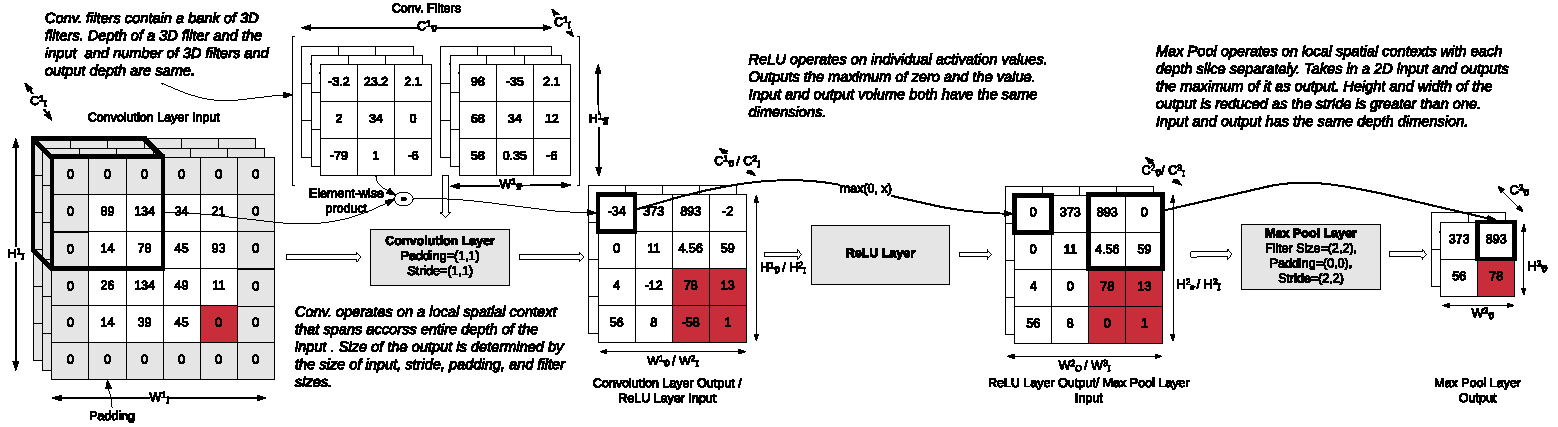
\includegraphics[width=\textwidth]{images/cnn_simplified}
\caption{Simplified representation of selected layers of a Deep CNN. For simplicity sake addition of bias is not shown in the Conv. transformation. The values marked in red shows how a small spatial update in the first input would propagate through subsequent transformations. Notation used is explained in Table ~\ref{table:preliminaries_symbols}.}
\end{figure*}

\begin{itemize}
	\item Transformations that operate on individual (point) spatial locations.
	\begin{itemize}
	 \item E.g. ReLU, Batch Normalization
	\end{itemize}
	\item Transformations that operate on a local spatial context.
	\begin{itemize}
	 \item E.g. Convolution, Pooling
	\end{itemize}
	\item Transformation that operate on the global spatial context.
	\begin{itemize}
	 \item E.g. Fully-Connected
	\end{itemize}
\end{itemize}

With incremental spatially localized modifications in the input, both types of transformations that operate at individual spatial locations and transformations that operate at a local spatial contexts provide opportunities for exploiting redundancy. Extending the transformations that operate at individual spatial locations to become redundancy aware is straightforward. However, with transformations that operate on a local spatial context such as convolution and pooling, this extension is non-trivial due to the overlapping nature of the spatial contexts corresponding to individual transformations. We next formally define the transformations of convolution and pooling layers and also the relationship between input and output dimensions for these layers which will be later used in Section. 4 to introduce our incremental inference approach.


\vspace{2mm}
\noindent \textbf{Transformations that operate on a local spatial context.} The two types of transformations that operate on a local spatial context in a deep CNN are convolution and pooling layers. Convolution layers are the most important type of layer in the CNN architecture which also contributes to most of the computational cost. Each convolutional layer can have several (say $C_{\mathcal{O}}$) three dimensional filter kernels organized into a four dimensional array $\mathcal{K}_{conv}$ with each having a smaller spatial width $W_\mathcal{K}$ and height $H_\mathcal{K}$ compared to the width $W_{\mathcal{I}}$ and height $H_{\mathcal{I}}$ of the input volume $\mathcal{I}$, but has the same depth $C_{\mathcal{I}}$. During inference, each filter kernel is slided along the width and height dimensions of the input and a two dimensional activation map is produced by taking element-wise product between the kernel and the input and adding a bias value $\mathcal{B}[c]$ for some c $\in$ $[0, C_{\mathcal{O}}-1]$. These two dimensional activation maps are then stacked together along the depth dimension to produce an output volume $\mathcal{O}$ having the dimensions of ($C_{\mathcal{O}}$,$H_{\mathcal{O}}$,$W_{\mathcal{O}}$). This can be formally defined as follows:

\begin{align}
\text{Input Volume}:&~ \mathcal{I} \in \mathcal{\rm I\!R}^{C_{\mathcal{I}} \times H_{\mathcal{I}} \times W_{\mathcal{I}}}\\
\text{Conv. Filters}:&~ \mathcal{K}_{conv} \in \mathcal{\rm I\!R}^{C_{\mathcal{O}} \times C_{\mathcal{I}} \times H_{\mathcal{K}} \times W_{\mathcal{K}}}\\
\text{Conv. Bias Vector}:&~ \mathcal{B}_{conv} \in \mathcal{\rm I\!R}^{C_{\mathcal{O}}}\\
\text{Output Volume}:&~ \mathcal{O} \in \mathcal{\rm I\!R}^{C_{\mathcal{O}} \times H_{\mathcal{O}} \times W_{\mathcal{O}}}
\end{align}

\begin{equation}
\label{eqn:conv_operator}
\begin{split}
\mathcal{O}[c,y,x] &= \sum_{k=0}^{C_{\mathcal{I}}} \sum_{j=0}^{H_\mathcal{K}-1} \sum_{i=0}^{W_\mathcal{K}-1} \mathcal{K}_{conv}[c, k, j, i] \\ & \quad \quad \quad \times \mathcal{I}[k,y-\floor{\frac{H_\mathcal{K}}{2}}+j,x-\floor{\frac{W_\mathcal{K}}{2}}+i] + \mathcal{B}[c]
\end{split}
\end{equation}

The main objective of having pooling layers in CNNs is to reduce the spatial size of output volumes. Pooling can also be thought as a convolution operation with a fixed (i.e. not learned) two dimensional filter kernel $\mathcal{K}_{pool}$ having a width of $W_\mathcal{K}$ and height of $H_\mathcal{K}$, which unlike convolution, operates independently on every depth slice of the input volume. The two main variations of pooling layers are max pooling (takes the maximum value from the local spatial context) and average (takes the average value from the local spatial context) pooling. A Pooling layer takes a three dimensional activation volume $\mathcal{O}$ having a depth of $C$, width of $W_{\mathcal{I}}$, and height of $H_{\mathcal{I}}$ as input and produces another three dimensional activation volume $\mathcal{O}$ which has the same depth of $C$, width of $W_{\mathcal{O}}$, and height of $H_{\mathcal{O}}$ as the output. Pooling kernel is generally slided with more than one pixel at a time and hence $W_{\mathcal{O}}$ and $H_{\mathcal{O}}$ are generally smaller than $W_{\mathcal{I}}$ and $H_{\mathcal{I}}$. Pooling operation can be formally defined as follows:

\begin{align}
\text{Pool Filters}:&~ \mathcal{K}_{pool} \in \mathcal{\rm I\!R}^{H_{\mathcal{K}} \times W_{\mathcal{K}}}
\end{align}

\begin{equation}
\label{eqn:pool_operator}
\begin{split}
\mathcal{O}[c,y,x] &= \sum_{j=0}^{H_\mathcal{K}-1} \sum_{i=0}^{W_\mathcal{K}-1} \mathcal{K}_{pool}[j, i] \\ & \quad \quad \quad \times \mathcal{I}[c,y-\floor{\frac{H_\mathcal{K}}{2}}+j,x-\floor{\frac{W_\mathcal{K}}{2}}+i]
\end{split}
\end{equation}


\vspace{2mm}
\noindent \textbf{Relationship between Input and Output Spatial Sizes.} The output volume's spatial size ($W_{\mathcal{O}}$ and $H_{\mathcal{O}}$) is determined by the spatial size of the input volume ($W_{\mathcal{I}}$ and $H_{\mathcal{I}}$), spatial size of the filter kernel ($W_\mathcal{K}$ and $H_\mathcal{K}$) and two other parameters: \textbf{stride} $S$ and \textbf{padding} $P$. Stride is the amount of pixel values used to slide the filter kernel at a time when producing a two dimensional activation map. It is possible to have two different values with one for the width dimension $S_x$ and one for the height dimension $S_y$. Generally $S_x \leq W_\mathcal{K}$ and $S_y \leq H_\mathcal{K}$. Sometimes in order to control the spatial size of the output activation map to be same as the input activation map, one needs to pad the input feature map with zeros around the spatial border. Padding ($P$) captures the amount of zeros that needs to be added. Similar to the stride $S$, it is possible to have two separate values for padding with one for the width dimension $P_x$ and one for the height dimension $P_y$. With these parameters defined the width and the height of the output activation volume can be defined as follows:

\begin{align}
W_{\mathcal{O}} = (W_{\mathcal{I}} - W_\mathcal{K} + 1 + 2\times P_x)/S_x \\
H_{\mathcal{O}} = (H_{\mathcal{I}} - H_\mathcal{K} + 1 + 2\times P_y)/S_y
\end{align}

\vspace{2mm}
\noindent \textbf{Estimating the Computational Cost of Deep CNNs}
Deep CNNs are highly compute intensive and out of the different types of layers, Conv layers contributes to $90\%$ (or more) of the computations. One of the widely used ways to estimate the computational cost of a Deep CNN is to estimate the number of fused multiply add (FMA) floating point operations (FLOPs) required by convolution layers for a single forward inference.
% and ignore the computational cost of other layers (e.g. Pooling, Fully-Connected).

For example, applying a convolution filter having the dimensions of ($C^l_{in}$, $H^l_{\mathcal{K}}$, $W^l_{\mathcal{K}}$) to a single spatial context will require $C^l_{\mathcal{I}} \times H^l_{\mathcal{K}} \times W^l_{\mathcal{K}}$ many FLOPs, each corresponding to a single element-wise multiplication. Thus, the total amount of computations $Q_l$ required by that layer in order to produce an output $\mathcal{O}$ having dimensions $C^l_{\mathcal{O}} \times H^l_{\mathcal{O}} \times W^l_{\mathcal{O}}$, and the total amount of computations $Q$ required to process the entire set of convolution layers $L$ in the CNN can be calculated as per equation.~\ref{eqn:full_local} and equation.~\ref{eqn:full_all}. However, in the case incremental updates effectively only a smaller spatial patch having a width $W^l_\mathcal{P}$ ($W^l_\mathcal{P}<=W^l_{\mathcal{O}}$) and height $H^l_\mathcal{P}$ ($H^l_\mathcal{P}<=H^l_{\mathcal{O}}$) is needed to be recomputed. The amount of computations required for the incremental computation $Q^l_{inc}$ and total amount of incremental computations $Q_{inc}$ required for the entire set of convolution layers $L$ will be smaller than the above full computation values and can be calculated as per equation.~\ref{eqn:inc_local} and equation.~\ref{eqn:inc_all}.

Based on the above quantities we define a new metric named \textbf{theoretical speedup ratio (R)}, which is the ratio between total full computational cost $Q$ and total incremental computation cost $Q_{inc}$ (see equation.~\ref{eqn:redundancy_ratio}). This ratio essentially acts as a surrogate for the theoretical upper-bound for computational and runtime savings that can be achieved by applying incremental computations to deep CNNs.

\begin{align}
\label{eqn:full_local}
Q^l =&~ (C^l_{\mathcal{I}} \times H^l_{\mathcal{K}} \times W^l_{\mathcal{K}}) \times (C^l_{\mathcal{O}} \times H^l_{\mathcal{O}} \times W^l_{\mathcal{O}})\\
\label{eqn:full_all}
Q =&~ \sum_{l \in L} Q^l\\
\label{eqn:inc_local}
Q_{inc}^l =&~ (C^l_{\mathcal{I}} \times H^l_{\mathcal{K}} \times W^l_{\mathcal{K}}) \times (C^l_{\mathcal{O}} \times H^l_{\mathcal{P}} \times W^l_{\mathcal{P}})\\
\label{eqn:inc_all}
Q_{inc} =&~ \sum_{l \in L} Q^l_{inc}\\
\label{eqn:redundancy_ratio}
R =&~ \frac{Q}{Q_{inc}}
\end{align}


\subsection{Estimating the Quality of Generated Approximate Heat Maps}

When applying approximate inference optimizations, \system~ sacrifices the the accuracy/quality of the generated heat map in favor of quicker execution.
To measure this drop of accuracy we use Structural Similarity (SSIM) Index~\cite{wang2004image}, which is one of the widely used approaches to measure the \textit{human perceived difference} between two similar images.
When applying SSIM index, we treat the original heat map as the reference image with no distortions and the perceived image similarity of the \system~generated heat map is calculated with reference to it.
The generated SSIM index is a value between $-1$ and $1$, where $1$ corresponds to perfect similarity.
% It is important to note that, even though SSIM index value of 1 corresponds to perfect similarity, other values doesn't necessarily imply same level of perceived quality across different image pairs.
% However, if the original images are closely similar, such as in chest X-ray images, it can be assumed that this condition will hold.
Typically SSIM index values above $0.95-0.80$ are used in practical applications such as image compression and video encoding as at the human perception level they produce indistinguishable distortions.
For more details on SSIM Index method, we refer the reader to the original SSIM Index paper~\cite{wang2004image}.